\subsection{Обоснование необходимости проводимого исследования}

\subsection{Организация и планирование работы}

Основные задачи организации и планирования работ:
\begin{itemize}
 \item определение объема предстоящих работ;
 \item определение основных этапов работ;
 \item установление сроков выполнения запланированных работ;
 \item определение необходимых денежных, материальных и трудовых ресурсов.
\end{itemize}


При выполнении дипломной работы были задействованы следующие лица:
\begin{itemize}
 \item руководитель (рук.);
 \item разработчик (разр.).
\end{itemize}

Месячный оклад студента, не являющегося дипломированным специалистом, составляет 2324,40 рублей.
С учетом 24 рабочих дней и 6-часового рабочего дня стоимость одного часа работ равна 16,14 рублей.
Месячный оклад руководителя с ученой степенью кандидата наук и должностью доцента составляет 14800 рублей.
Стоимость одного часа работ с учетом 24-ех 6-часовых рабочих дней равна 102,78 рублей.   

Руководитель работы оказывает помощь разработчику в планировании работ в период проектирования, рекомендует
необходимую литературу, проводит консультации разработчика, осуществляет контроль над выполнением всех 
намеченных этапов работы. Разработчик реализует объем работ, установленный в техническом задании.

График работ приведен в таблице~\ref{tab:job_is_done_1}.

\begin{table}[!ht]
\caption{График выполнения работ}
\centering
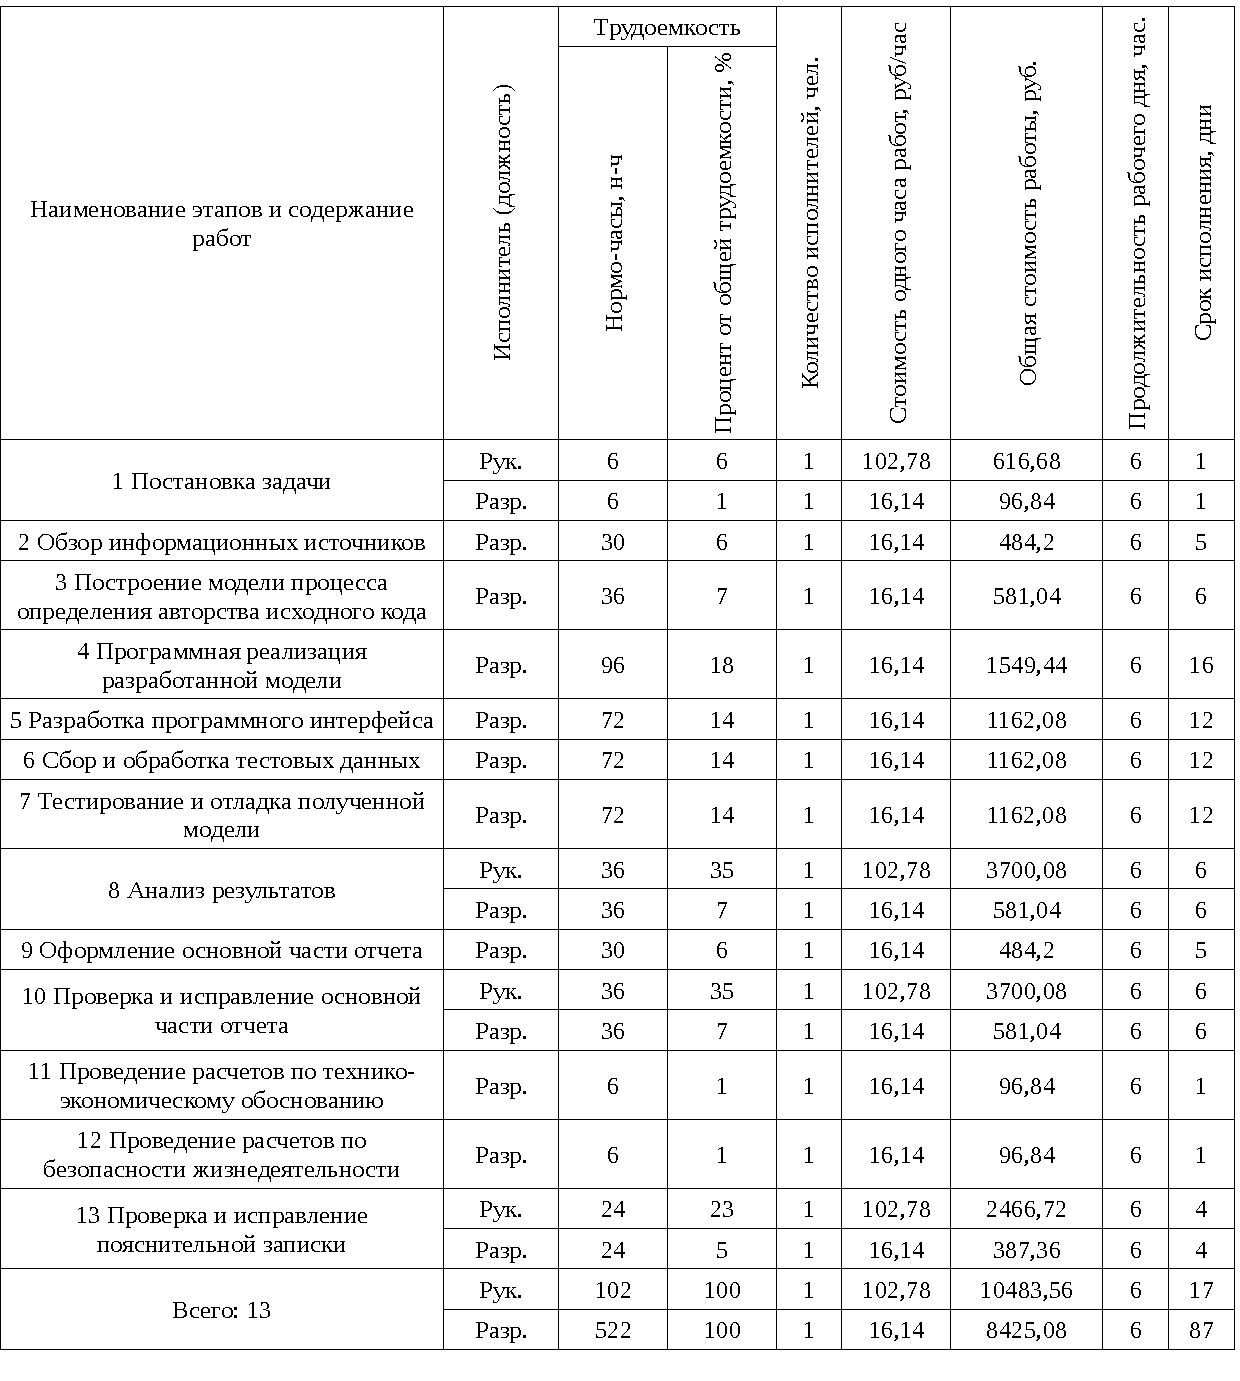
\includegraphics[page=1, width=1\linewidth]{schedule.pdf}
\label{tab:job_is_done_1}
\end{table}


\begin{table}[!ht]
\caption{Ленточный график загрузки участников работ}
\centering
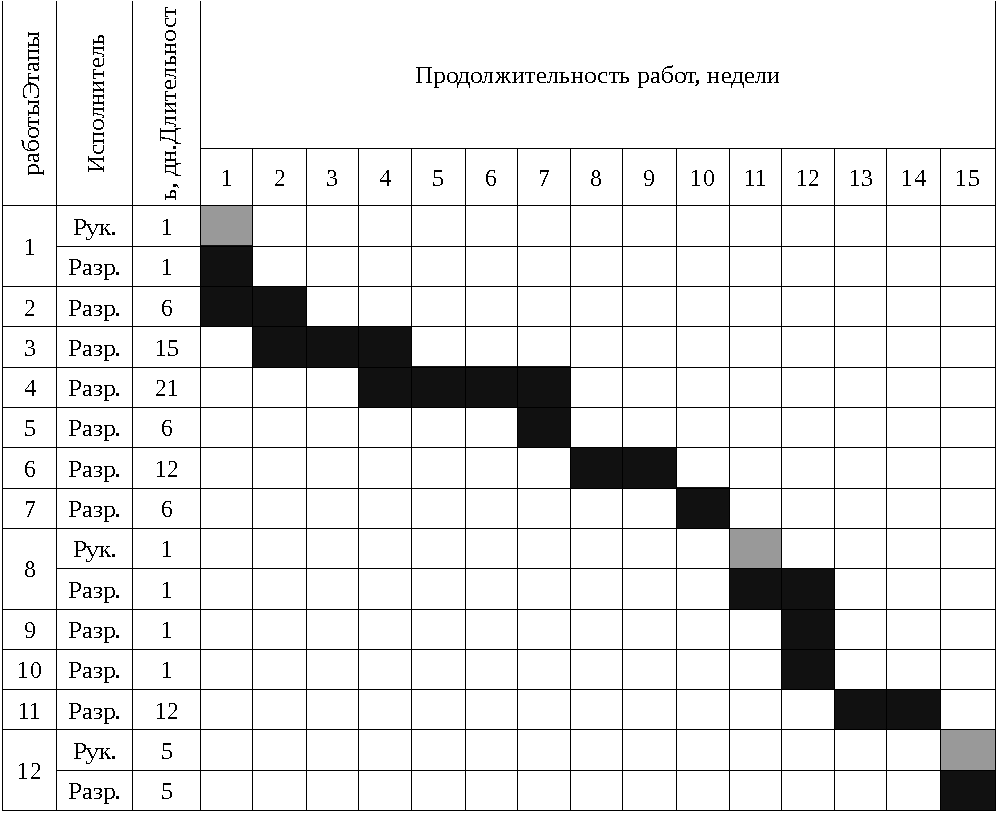
\includegraphics[page=1, width=1\linewidth]{schedule_2.pdf}
\label{tab:job_is_done_2}
\end{table}

\begin{table}[!ht]
\caption{Календарный график загрузки участников}
\centering
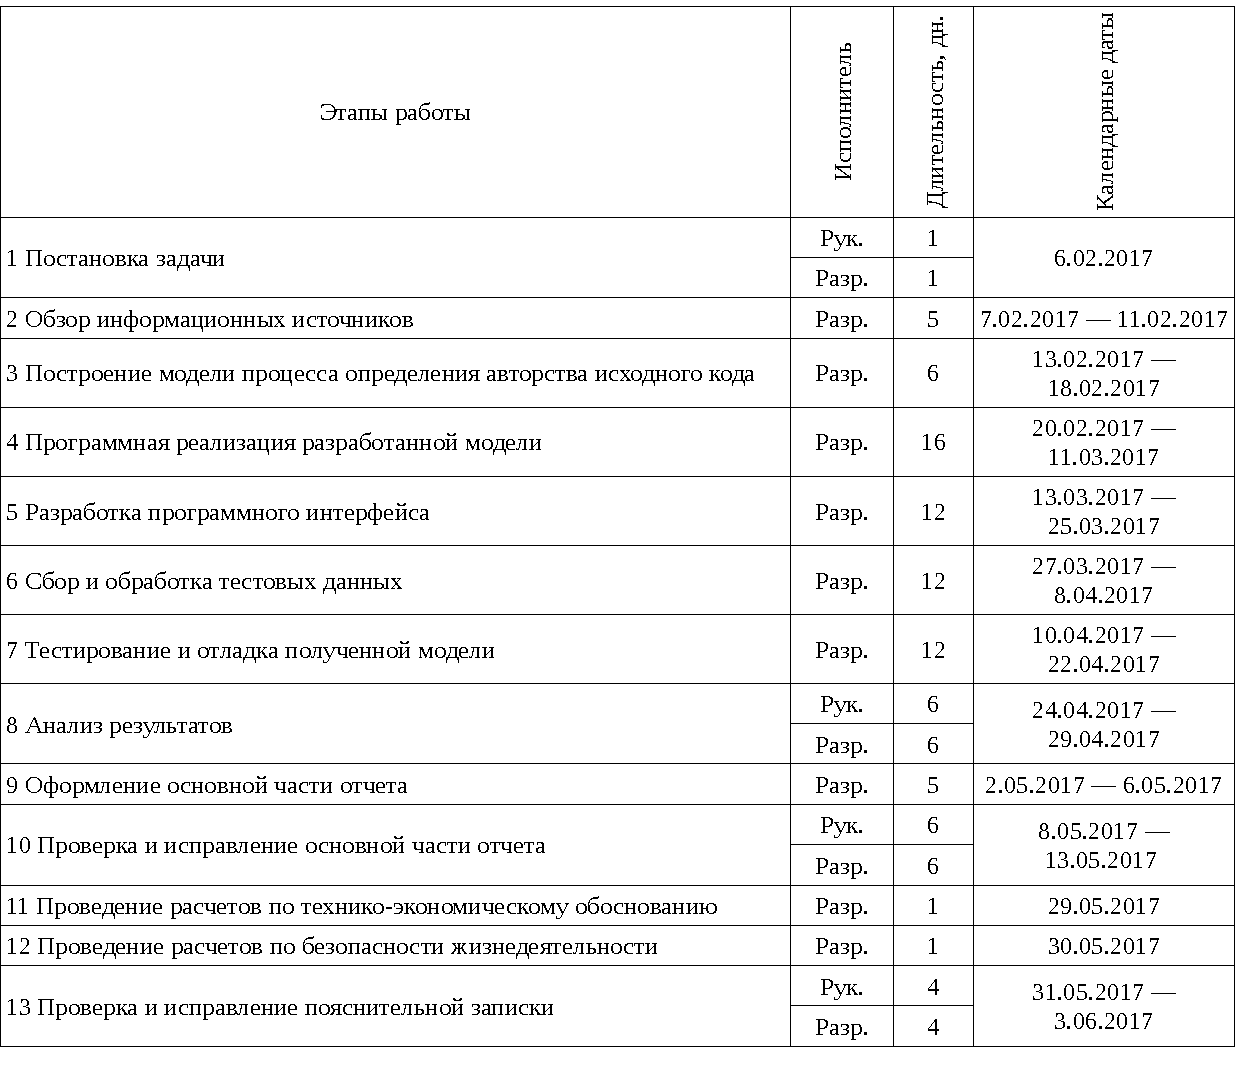
\includegraphics[page=1, width=1\linewidth]{schedule_3.pdf}
\label{tab:job_is_done_3}
\end{table}

\begin{table}[!ht]
\caption{Смета затрат на оборудование}
\centering
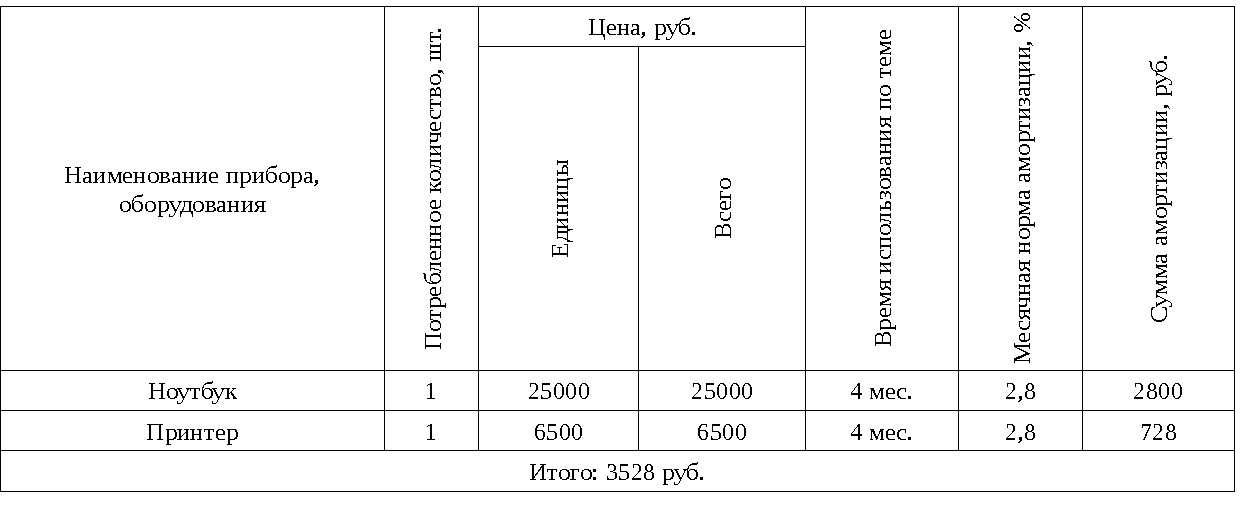
\includegraphics[page=1, width=1\linewidth]{schedule_4.pdf}
\label{tab:job_is_done_4}
\end{table}

\begin{table}[!ht]
\caption{Расчет расходов на оплату труда участников проекта}
\centering
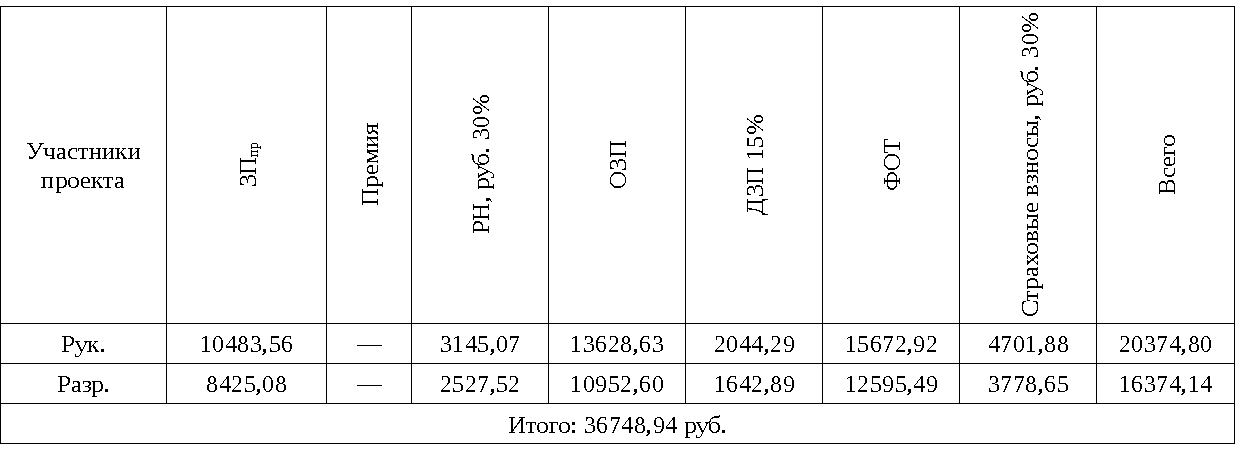
\includegraphics[page=1, width=1\linewidth]{schedule_5.pdf}
\label{tab:job_is_done_5}
\end{table}


\subsubsection{Затраты на основные и вспомогательные материалы}

Статья включает расходы по приобретению и доставке основных и вспомогательных материалов, необходимых для опытно-экспериментальной проработки решения, для изготовления макета или опытного оборудования. Сюда включаются и стоимость необходимых материалов для изготовления образцов и макетов, и материалов необходимых для оформления требуемой документации.

Размер транспортно-заготовительных расходов (ТЗР), определяемый в процентах от стоимости, примем 10\%. Стоимость вспомогательных материалов принимается 10\% от стоимости основных материалов с учётом ТЗР. Результаты расчёта стоимости материалов представлены в \ref{tab:eco_6}.

\begin{table}[!ht]
\caption{Расчёт затрат на основные и вспомогательные материалы}
\centering
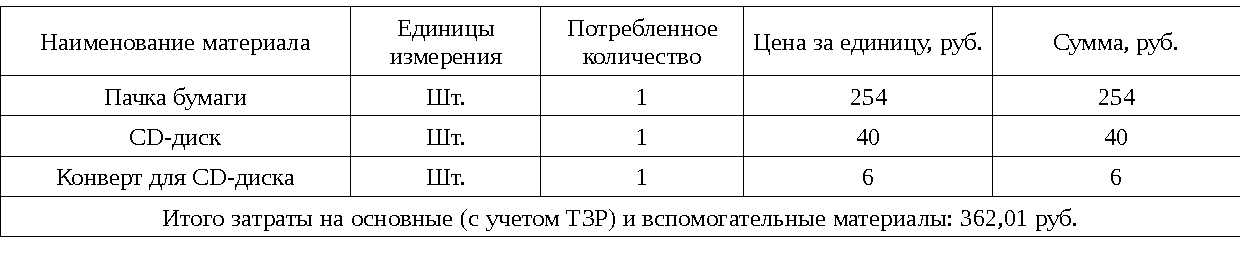
\includegraphics[page=1, width=1\linewidth]{econom.pdf}
\label{tab:eco_6}
\end{table}


\subsubsection{Расходы на электроэнергию}

Статья включает затраты по электроэнергии на технологические нужды. В настоящее время тариф на электроэнергию для населения г. Томска на 2017 год составляет 2,17 руб./ кВт ч. Тариф введен 
приказом от 23.12.2016 г. \textnumero~6-840 <<О тарифах на электрическую энергию для населения и 
потребителей, приравненных к категории население по Томской области на 2017 год>>, 
принятый департаментом тарифного регулирования Томской области.

Результаты расчётов приведены в \ref{tab:eco_7}.

\begin{table}[!ht]
\caption{Затраты на электроэнергию}
\centering
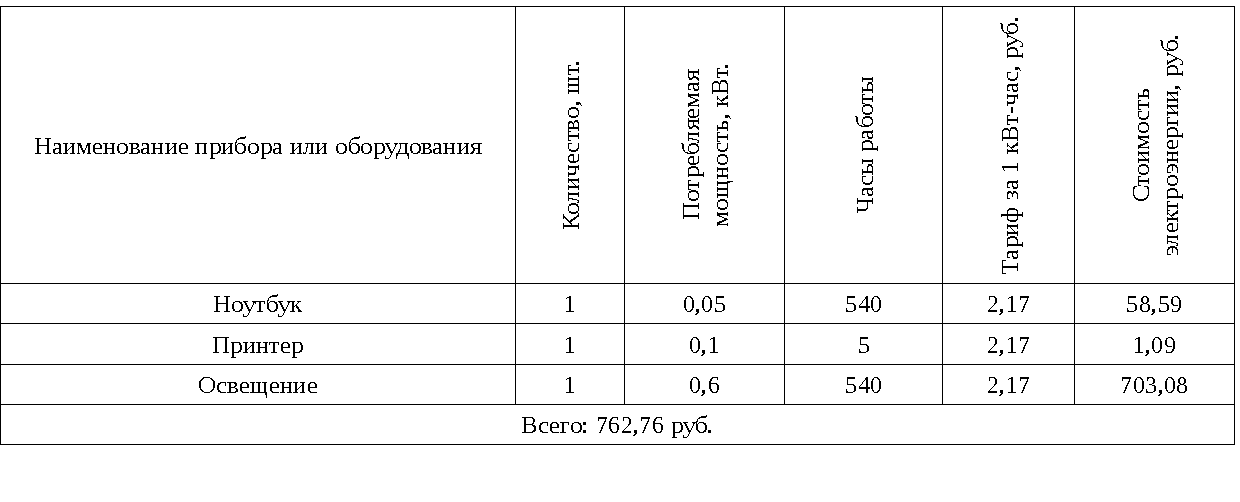
\includegraphics[page=1, width=1\linewidth]{econom_2.pdf}
\label{tab:eco_7}
\end{table}

\subsubsection{Накладные расходы}

Расчёт накладных расходов сведём в \ref{tab:eco_8}.

\begin{table}[!ht]
\caption{Накладные расходы}
\centering
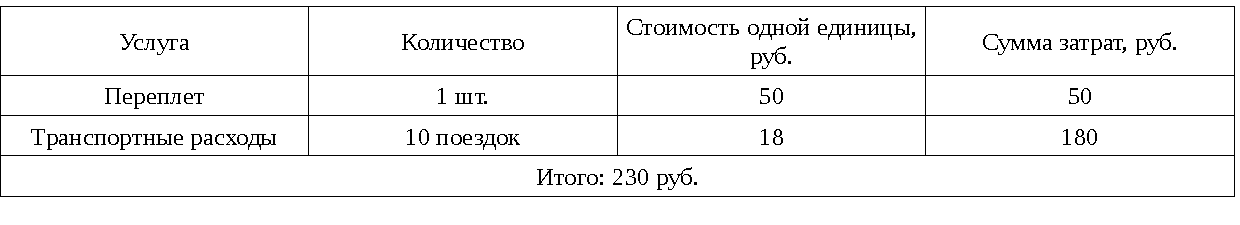
\includegraphics[page=1, width=1\linewidth]{econom_3.pdf}
\label{tab:eco_8}
\end{table}

\subsubsection{Сводная смета затрат}

На основании всех произведённых расчётов составим сводную смету затрат на выполнение работы в виде таблицы \ref{tab:eco_9}.

\begin{table}[!ht]
\caption{Сводная смета затрат}
\centering
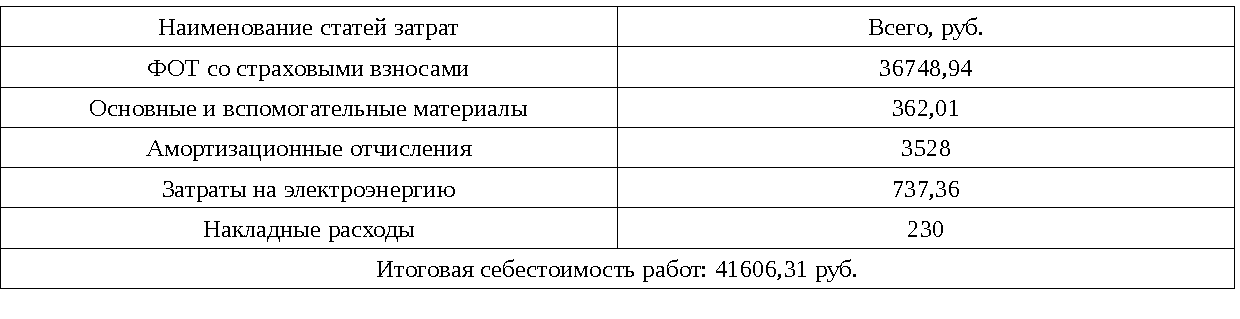
\includegraphics[page=1, width=1\linewidth]{econom_4.pdf}
\label{tab:eco_9}
\end{table}

\subsection{Научно-технический эффект}
Количественная оценка научно-технического уровня может быть произведена путём расчёта результативности участников разработки по формуле:
$$K_{\textit{ну}} = \sum_{i=1}^{n}(K_{\textit{ду}}\cdot d_{i}),$$
где\ $K_\textit{ну}$ – коэффициент научного или научно-технического уровня;\\$K_\textit{дуi}$ – коэффициент достигнутого уровня $\textit{i}{}$-го фактора;\\$d_{i}$– значимость $i$-го фактора;\\$\textit{n}$ – количество факторов.

Весовые коэффициенты \textit{d} для каждого из факторов устанавливались экспертным путём. При этом сумма коэффициентов значимости по всем факторам равна единице. Коэффициенты достигнутого уровня факторов также установлены экспертным путём.

\begin{table}[!ht]
\caption{Оценка научно-технического уровня разработки}
\centering
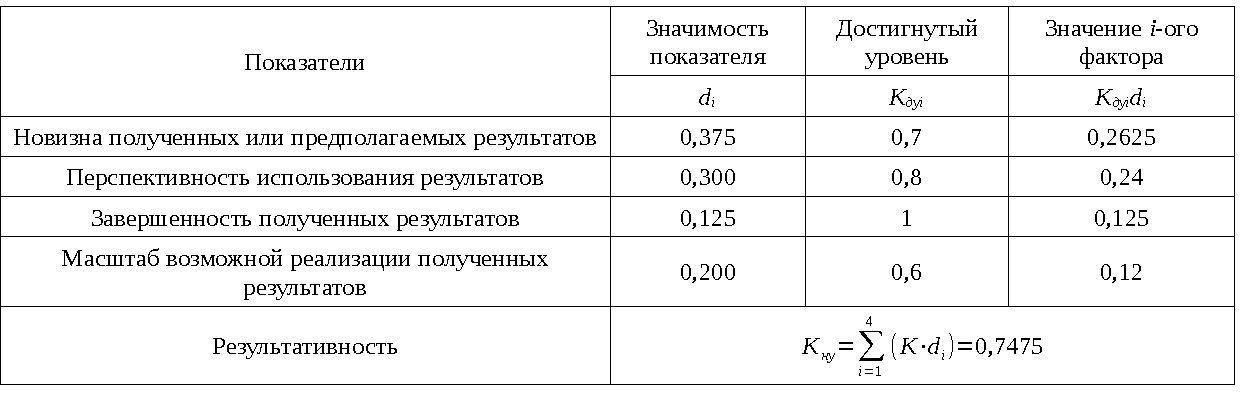
\includegraphics[page=1, width=1\linewidth]{econom_5.pdf}
\label{tab:eco_10}
\end{table}
Рассчитанный коэффициент научно-технической результативности равен 0,7475. Полученное значение достаточно высоко, что говорит об эффективности проведённых работ выше среднего, однако отмечается необходимость дальнейшего развития проекта для достижения завершённости полученных результатов.

\subsection{Социальный эффект}



\clearpage